%\section{Implémentation}    
\chapter{Implémentation}
\markboth{\MakeUppercase{Implémentation}}{}
	
	\section{Choix algorithmiques}

		\subsection{Calcul des zones d'influence}
		
			\paragraph{}
			Le calcul des zones d'influence est découpé en 2 fonctions distinctes :
			
			\paragraph{1. runInfluenceArea : }
			Cette fonction se charge de récupérer toutes les unités mobiles d'un Board qui lui est passé en paramètre.
			Elle lance ensuite computeInfluenceAreas sur chacune de ces unités.
			[Code de la fonction]
			
			\paragraph{2. computeInfluenceAreas : }
			Cette fonction récursive calcule la zone d'influence pour une unité donnée à partir d'une case et d'une variable speedLeft. 
			(qui correspond à la capacité de déplacement restante de l'unité)
			Si la capacité de déplacement restante d'une unité n'est pas nulle (speedLeft\textgreater0), alors on parcoure toutes les cases 
			qui sont autour de la case passée en paramètre. 
			Au premier appel de cette fonction, cette case sera la case sur laquelle se situe l'entité pour laquelle on calcule la zone d'influence.
			Si une ou plusieurs de ces cases sont libres, on modifie l'entité en ajoutant ces cases dans la liste de ses mouvements possibles, 
			puis on rappelle computeInfluenceAreas sur celles-ci en décrémentant le speedLeft de 1.
			Ainsi La zone d'influence ne pourra pas s'étendre à travers les unités ou les montagnes.
			[Code de la fonction]
		
		\subsection{Calcul des communications}
		
			La propagation des communications est découpés en 2 fonctions distinctes :
			
			\paragraph{1. computeArsenalsCommunications : }
			Cette fonction se charge de calculer les communications pour l'ensemble des arsenaux se trouvant sur le Board.
			Elle récupère donc l'ensemble des arsenaux sur le plateau et appelle la fonction computeCommunications sur chacun d'entre eux.
			
			\paragraph{2. computeCommunications : }
			Chaque fois qu'une entité propageant des communications est trouvée, (donc arsenal ou relais en communication) cette fonction est appelée
			avec les coordonnées x et y de l'unité en question.
			N'importe quelle unité propageant les lignes de communication le fait dans 8 directions. (nord, nord-est, est, etc)
			Nous parcourons donc ces 8 lignes une à une, case par case et ajoutons toutes les cases libre à la liste des communications jusqu'à
			la rencontre d'un obstacle. (Montagne, unités adverse ou bien fin du plateau)
			Par la suite, si Drools détecte qu'un nouveau relais est connecté suite à la propagation de lignes de communications, computeCommunications
			sera ré-appelée sur ces relais nouvellement connectés.
		
		\subsection{Calcul des potentiels}
		
			\paragraph{}
			Le calcul des potentiels est découpé en 3 fonctions distinctes :
			
			\paragraph{1. computePotentials : }
			Cette fonction se charge de remplir la matrice des potentiels pour chaque équipe.
			Elle parcoure le board dans son intégralité (une fois pour chaque équipe), appelle sur chaque case les fonctions computeAttack et 
			computeDefence, puis enregistre les valeurs dans une matrice.
			
			\paragraph{2. computeDefence : }
			Cette fonction calcule la défense pour une case et une équipe donnée.
			Après avoir initialisé la defense à 0, nous parcourons une à une les lignes pouvant avoir un impact sur la défense d'une unité.
			Il y a donc 8 lignes distinctes. (ligne au nord de l'unité, ligne au nord-est, ligne à l'est, etc)
			Pour chaque ligne, nous parcourons ensuite chaque case de la plus proche à la plus lointaine.
			Si une de ces cases contient une unité alliée à portée, nous ajoutons la défense de cette unité à la défense de cette case, 
			sauf dans le cas ou nous avons rencontré un obstacle.
			Pour savoir si nous avons rencontré un obstacle, nous mettons simplement le booléen obstacle à true si une des cases de la 
			ligne contient une unité ennemie ou une montagne.
			
			\paragraph{3. computeAttack : }
			Cette fonction calcule l'attaque subie pour une case et une équipe donnée.
			Elle a un fonctionnement très similaire à computeDefence, excepté que nous avons du ici prendre en compte la charge pour les cavaleries. 
			(qui est d'ailleurs annulée dés lors qu'un cavalier se situe sur un fort)
			Pour prendre en compte ceci, nous avons rajouté un booléen charge qui est passé à false quand on rencontre un obstacle 
			ou un fort sur la ligne analysée.
			La valeur d'attaque varie suivant si le cavalier est en charge ou non donc nous ajoutons attackCharge si le booléen charge est 
			à true ou attack si le booléen est à false.
			
		\clearpage
	 

	\section{Tests réalisés}

		\subsection{Tests de non-régression}
		
		Afin d'éviter la régression lors de l'évolution du projet nous avons utilisé la librairie JUnit pour faciliter la gestion des tests. 
		Nous avons généré des classes de tests afin de valider le bon fonctionnement de l'ensemble des méthodes pour une classe donnée.
		Par soucis de temps, nous n'avons pas pu réaliser les tests pour chaque classes du projet, nous avons donc décidé de ne faire ces tests que sur les classes les plus « critiques ».\\ \\
		Parmis ces classes dites « critiques » nous avons la classe {\itshape EntityLoader} qui est garantie le bon placement des unités ainsi que la classe Board qui contient les données du jeu
		ainsi que certains algorithmes principaux.
		\\ \\
		Après chaque modification du code nous pouvons lancer tous nos tests afin de vérifier que les changements apportés n'ont pas altérés le fonctionnement du code précédent.
		
		\subsection{Tests unitaires}

			\subsubsection{EntityLoader}
				
				Afin de tester cette classe nous avons créé 9 tests, parmis ces tests nous en avons 2 pour tester les constructeurs et 2 pour tester les setters.\\ \\
				La méthode {\itshape isValidFormat(String[] line)} permet de vérifier qu'une ligne d'un fichier chargé respecte le bon format.
				Pour tester cette méthode nous lui passons en paramètre une ligne invalide et nous vérifions que {\itshape isValidFormat} nous retourne {\itshape false}.
				Ensuite nous testons avec un paramètre respectant le format et nous vérifions que la méthode retourne {\itshape true}.\\ \\

				La méthode {\itshape isValidFileFormat(String file)} permet de vérifier, en faisant appel à {\itshape isValidFormat}, que l'ensemble du fichier possède le bon format.
				Un premier test permet de vérifier que la méthode retourne {\itshape true} si on passe en paramètre un fichier au format correct.
				Le deuxième test consiste à passer en paramètre un fichier au format incorrect et vérifier que la méthode retourne {\itshape false}.\\ \\

				Pour tester si une exception est levée si il y a une tentative de chargement de fichier incorrect nous essayons de charger un fichier au format incorrect.
				Nous utilisons une annotation proposée par JUnit 4, pour vérifier qu'une exception est bien levée, dont voici le code : 
				
				\begin{lstlisting}[frame=single]
@Test(expected = BoardFileFormatException.class)
				\end{lstlisting}

				\begin{figure}[!h]
				    \caption{Résultats des tests de la classe EntityLoader}
				    \centerline{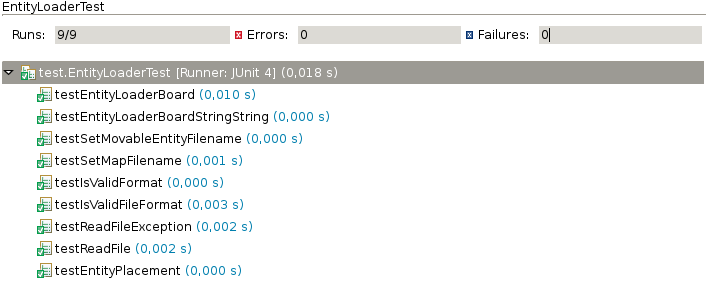
\includegraphics[scale=0.7]{images/tests_unitaires/entityloader.png}}
				\end{figure}

				
		\subsection{Tests fonctionnels}
		
			\subsubsection{Chargement d'un fichier incorrect}
				L'utilisateur est libre de pouvoir charger une partie en utilisant un fichier pour charger les éléments statiques (montagne, arsenal, forteresse, col) et un autre fichier pour charger les unités (infanterie, cavalier, ...). Etant donné que nous utilisons un format particulier pour que notre chargeur puisse lire les informations contenues dans ces fichiers, il faut donc vérifier que le format est bon pour éviter tout problème.
				\\ \\
				Dans ce test nous allons voir ce qu'il se passe si l'on décide de charger un fichier dont le format ne correspond pas au format attendu par notre chargeur.
				Nous essayons de charger le fichier {\itshape ErrSample.ksv} dont la dernière ligne est la suivante {\itshape WrongName;1;10;11}. 

				\begin{figure}[!h]
				    \caption{Chargement d'un fichier incorrect}
				    \centering
				    \centerline{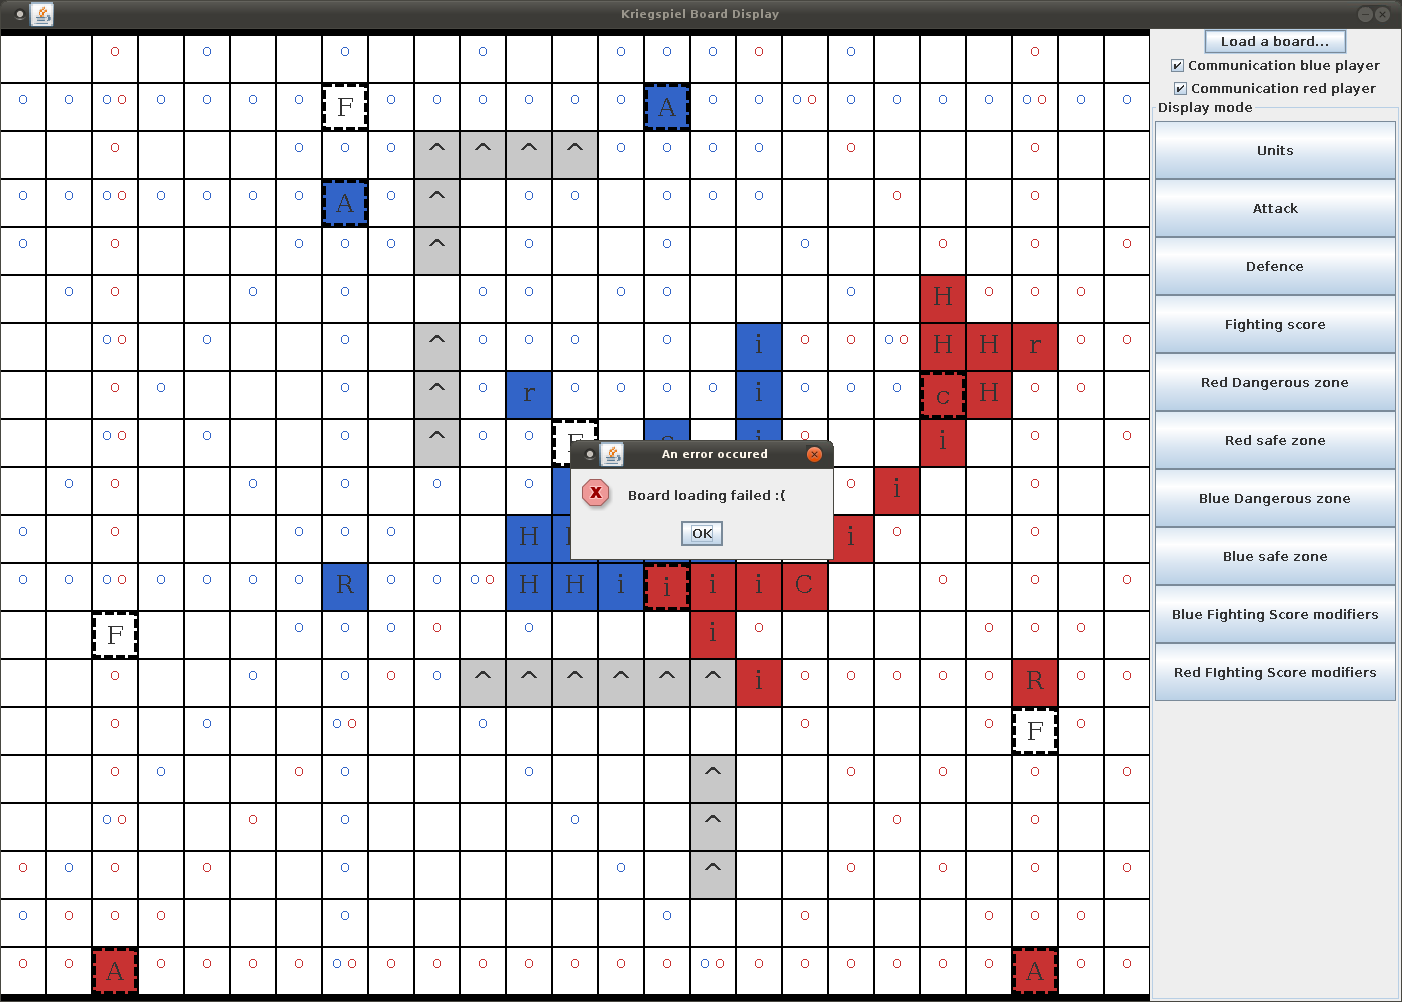
\includegraphics[scale=0.35]{images/tests_fonctionnels/incorrect_file.png}}
				\end{figure}

				\paragraph{Résultat\\}
					Un message d'erreur apparait à l'écran pour nous indiquer que le fichier n'a pas pu être chargé et le plateau reste inchangé.
					Ce test est validé dans la mesure où cela ne provoque pas de disfonctionnement mais l'utilisateur est informé du problème.

			\subsubsection{Représentation d'une situation}
				Un de nos besoins fonctionnels était de pouvoir représenter une situation de jeu pour tester cela on lance notre application et nous chargeons une partie.

				\begin{figure}[!h]
				    \caption{Représentation d'une situation}
				    \centerline{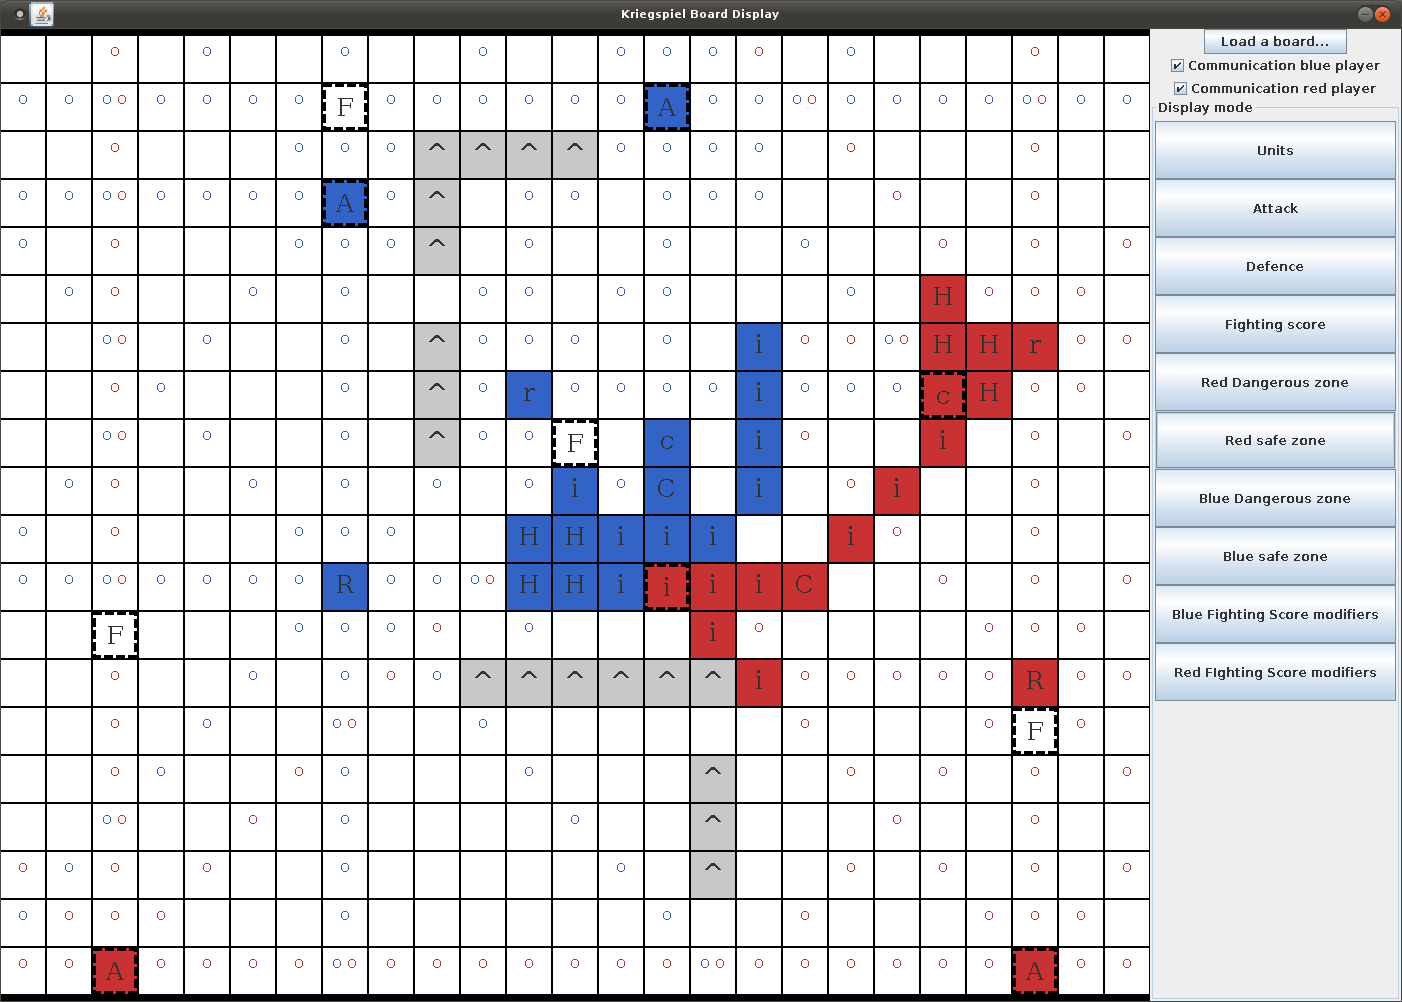
\includegraphics[scale=0.35]{images/tests_fonctionnels/representation_situation.png}}
				    \label{fig:representation_situation}
				\end{figure}

				\paragraph{Résultat\\}
					On voit sur la figure~\ref{fig:representation_situation} les différentes entités du jeu représentées par différents symboles.
					L'information de la partie est affichée à l'écran nous pouvons donc dire que ce test est validé.


			\subsubsection{Affichage de la zone d'influence}
				Un autre besoin fonctionnel était l'intégration des règles du jeu dans notre moteur de règles. Dans ce test nous allons vérifier que la zone d'influence affichée est correcte. Pour cela nous chargeons une partie et lors du clic sur une unité nous obtenons le résultat visible ci-dessous.

				\begin{figure}[!h]
				    \caption{Affichage de la zone d'influence}
				    \centerline{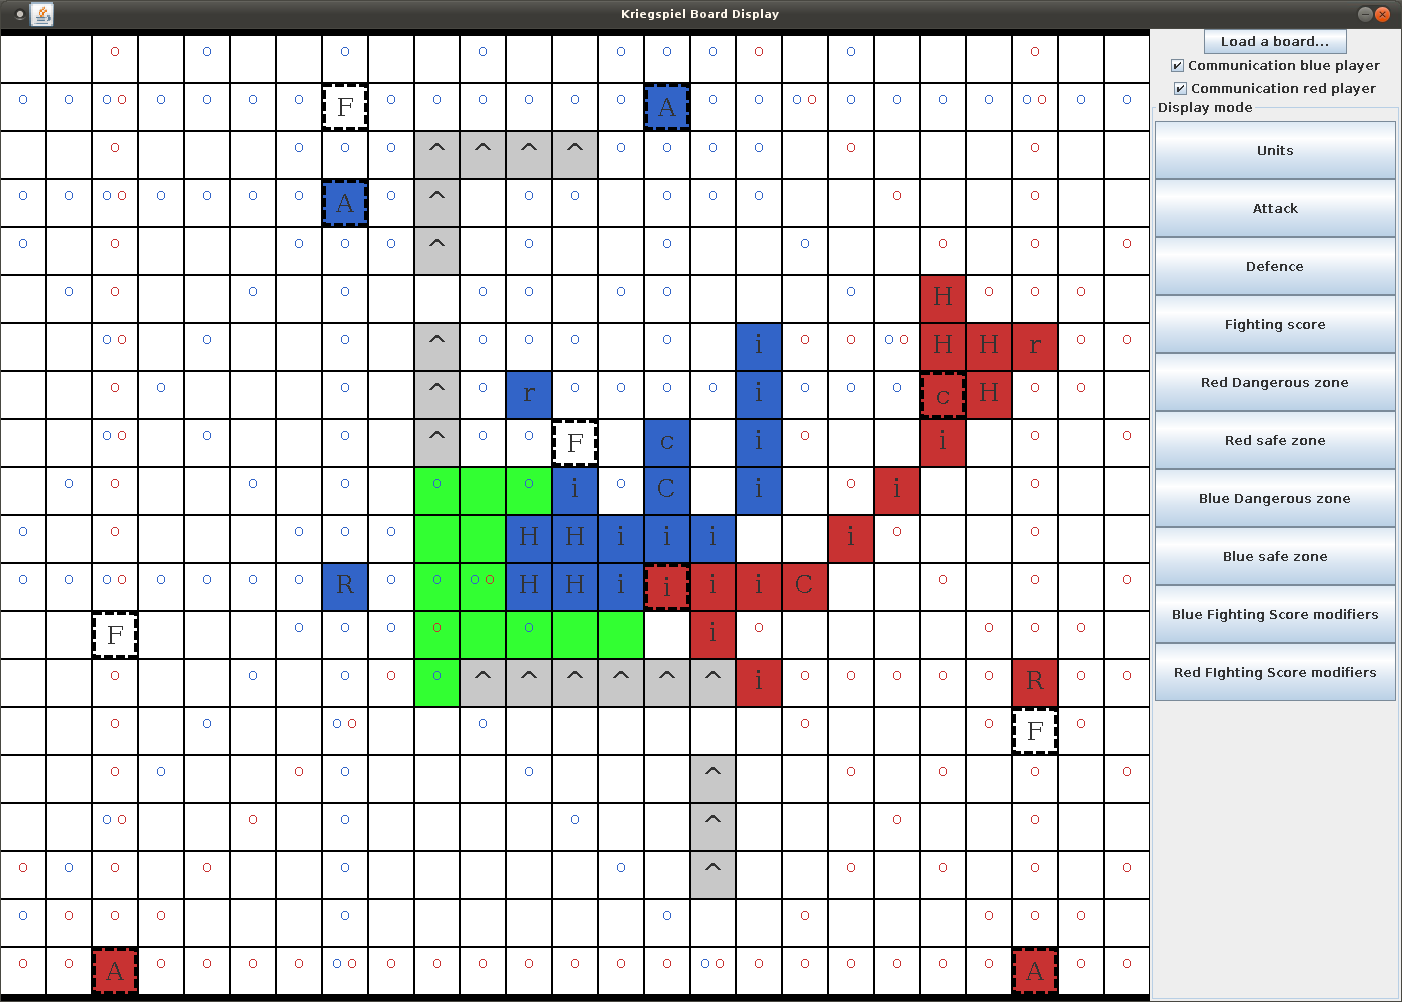
\includegraphics[scale=0.35]{images/tests_fonctionnels/zone_influence.png}}
				    \label{fig:affichage_zone_influence}
				\end{figure}

				\paragraph{Résultat\\}
					Les cases avec un fond vert sont les cases sur lesquelles peuvent se déplacer l'unité selectionnée. Sur la figure~\ref{fig:affichage_zone_influence} un cavalier a été selectionné, nous constatons que la zone d'influence est en accord avec la règle spécifiant qu'un cavalier peut se déplacer de 2 cases. 
					
			\subsubsection{Autres tests}
			
				Nous avons créé 15 classes de test permettant de tester un total de 68 méthodes, qui sont les plus importantes pour le bon fonctionnent de notre projet.
				Tous ces tests nous ont permis de détecter certaines erreurs que nous avons bien sûr corrigé.
				Ne pouvant évidemment pas présenter l'ensemble de ces tests dans le rapport, nous vous invitons à parcourir les différentes classes de test existantes.
